\documentclass[10pt,twocolumn]{article}

% --- PACKAGES ---
\usepackage[utf8]{inputenc}
\usepackage[margin=0.75in]{geometry}
\usepackage{amsmath,amssymb,amsfonts}
\usepackage{graphicx}
\usepackage{booktabs}
\usepackage{tabularx}
\usepackage{xcolor}
\usepackage{hyperref}
\usepackage{cite}
\usepackage{microtype}
\usepackage{caption}
\usepackage{subcaption}

\hypersetup{
    colorlinks=true,
    linkcolor=teal,
    citecolor=teal,
    urlcolor=teal
}

% --- TITLE & AUTHORS ---
\title{\textbf{AegisMed: Making Clinical Decision Support Reliable Through Active Questioning, Evidential Conflict Resolution, and Conformal Risk Bounding}}

\author{
    \textbf{Arham Saghir}$^{1}$ \quad \textbf{AegisMed Research Initiative Contributors}$^{1}$ \\
    $^{1}$Department of Computer Science and Engineering \\
    \texttt{\{arham.saghir\}@acm.org}
}

\date{October 2026}

\begin{document}

\maketitle

% --- ABSTRACT ---
\begin{abstract}
\noindent When people use artificial intelligence for medical advice, current systems usually suffer from three practical flaws. First, they try to guess a diagnosis from a single prompt without asking follow-up questions, which leads to vague or premature conclusions. Second, when clinical text and medical images disagree, standard models often average their outputs or hallucinate a consensus that violates basic biology. Third, standard neural networks output overconfident confidence scores without statistical guarantees. We built \textbf{AegisMed} to solve these three problems through four clear mechanisms:
(1) \textbf{Dynamic Entropy-Minimizing Active Triage (DEMAT)}, which tracks diagnostic uncertainty as Shannon entropy and actively selects the single best clinical question that clears up the most confusion;
(2) \textbf{Evidential Neuro-Symbolic Conflict Arbitration (EN-SCAF)}, which translates outputs from text, vision, and vitals models into Dempster-Shafer belief masses and measures direct disagreement with a conflict metric $K$;
(3) an \textbf{Ontological Knowledge Gate}, which consults the Unified Medical Language System (UMLS) and SNOMED-CT knowledge graphs whenever models clash ($K > 0.40$), discarding biologically impossible disease candidates before combining evidence; and
(4) \textbf{Multimodal Conformal Risk Bounding}, which generates a small set of plausible diagnoses mathematically guaranteed to contain the patient's true condition at least 95\% of the time ($1 - \alpha = 0.95$).
We evaluated AegisMed on 200 standardized clinical cases spanning 15 disease categories. Active questioning increased Top-1 diagnostic accuracy from 93.0\% to \textbf{98.0\%} ($+5.0\%$, $p = 0.0339$), attained \textbf{100.0\% Top-3 differential coverage}, and cut diagnostic uncertainty by \textbf{53.7\%} (from 2.846 down to 1.318 bits). The system achieved this while asking an average of only \textbf{1.92 questions per case} with an optimization latency of \textbf{0.2 ms}. Furthermore, expected calibration error fell from 0.5528 to 0.2451 ($-55.7\%$), showing that active inquiry makes clinical AI substantially more accurate, cautious, and trustworthy.
\end{abstract}

% --- SECTION 1: INTRODUCTION ---
\section{Introduction}

Diagnostic error remains a leading cause of preventable adverse events and diagnostic delays in outpatient and emergency medicine \cite{johnson2019mimic}. When a patient walks into a clinic complaining of chest pain, an experienced doctor never makes an immediate diagnosis. The phrase ``chest pain'' could point to a life-threatening heart attack, an acute case of pneumonia, or simple acid reflux. Instead of guessing, the doctor immediately asks targeted follow-up questions: Does the pain get worse with exertion? Does it radiate down your left arm? Does it hurt when you take a deep breath? Each answer narrows down the possibilities and rules out dangerous alternatives.

Current conversational AI models and clinical decision support tools rarely work this way. Most commercial systems operate as passive text engines: they take whatever summary the patient typed in a single prompt and output an immediate list of potential diseases. In acute medical triage, this passive approach breaks down in three distinct ways:

\begin{enumerate}
    \item \textbf{Single-Prompt Guesswork vs. Interactive Clarification:} Real clinical consultations are conversations, not one-way monologues. Static AI prompts cannot ask targeted follow-up questions to distinguish look-alike conditions. When symptoms overlap, single-turn models frequently guess the most common disease or give an unhelpfully broad list of possibilities.
    \item \textbf{Silent Contradictions Between Data Types:} Real patient cases involve text notes, vital signs, and diagnostic imaging. A chest X-ray model might see a cloudy patch in the lung and suspect pneumonia, while a text model focuses on mild stomach burning and suggests gastritis. When AI systems simply average their numerical scores, they blur this disagreement together, sometimes producing a smooth explanation for a combination of conditions that makes no medical sense.
    \item \textbf{Misleading Confidence Scores:} Deep learning models are notorious for producing overconfident softmax probabilities. A system might claim it is ``95\% confident'' in an incorrect diagnosis. In healthcare, clinicians cannot rely on arbitrary percentages; they need statistical guarantees that bound the risk of missing a patient's true illness.
\end{enumerate}

To address these challenges, we created \textbf{AegisMed}, a practical multi-agent clinical decision support system. Instead of viewing diagnosis as a text generation task, AegisMed treats triage as an interactive process of removing diagnostic doubt, cross-checking evidence across modalities, and bounding risk.

\begin{figure*}[t!]
\centering
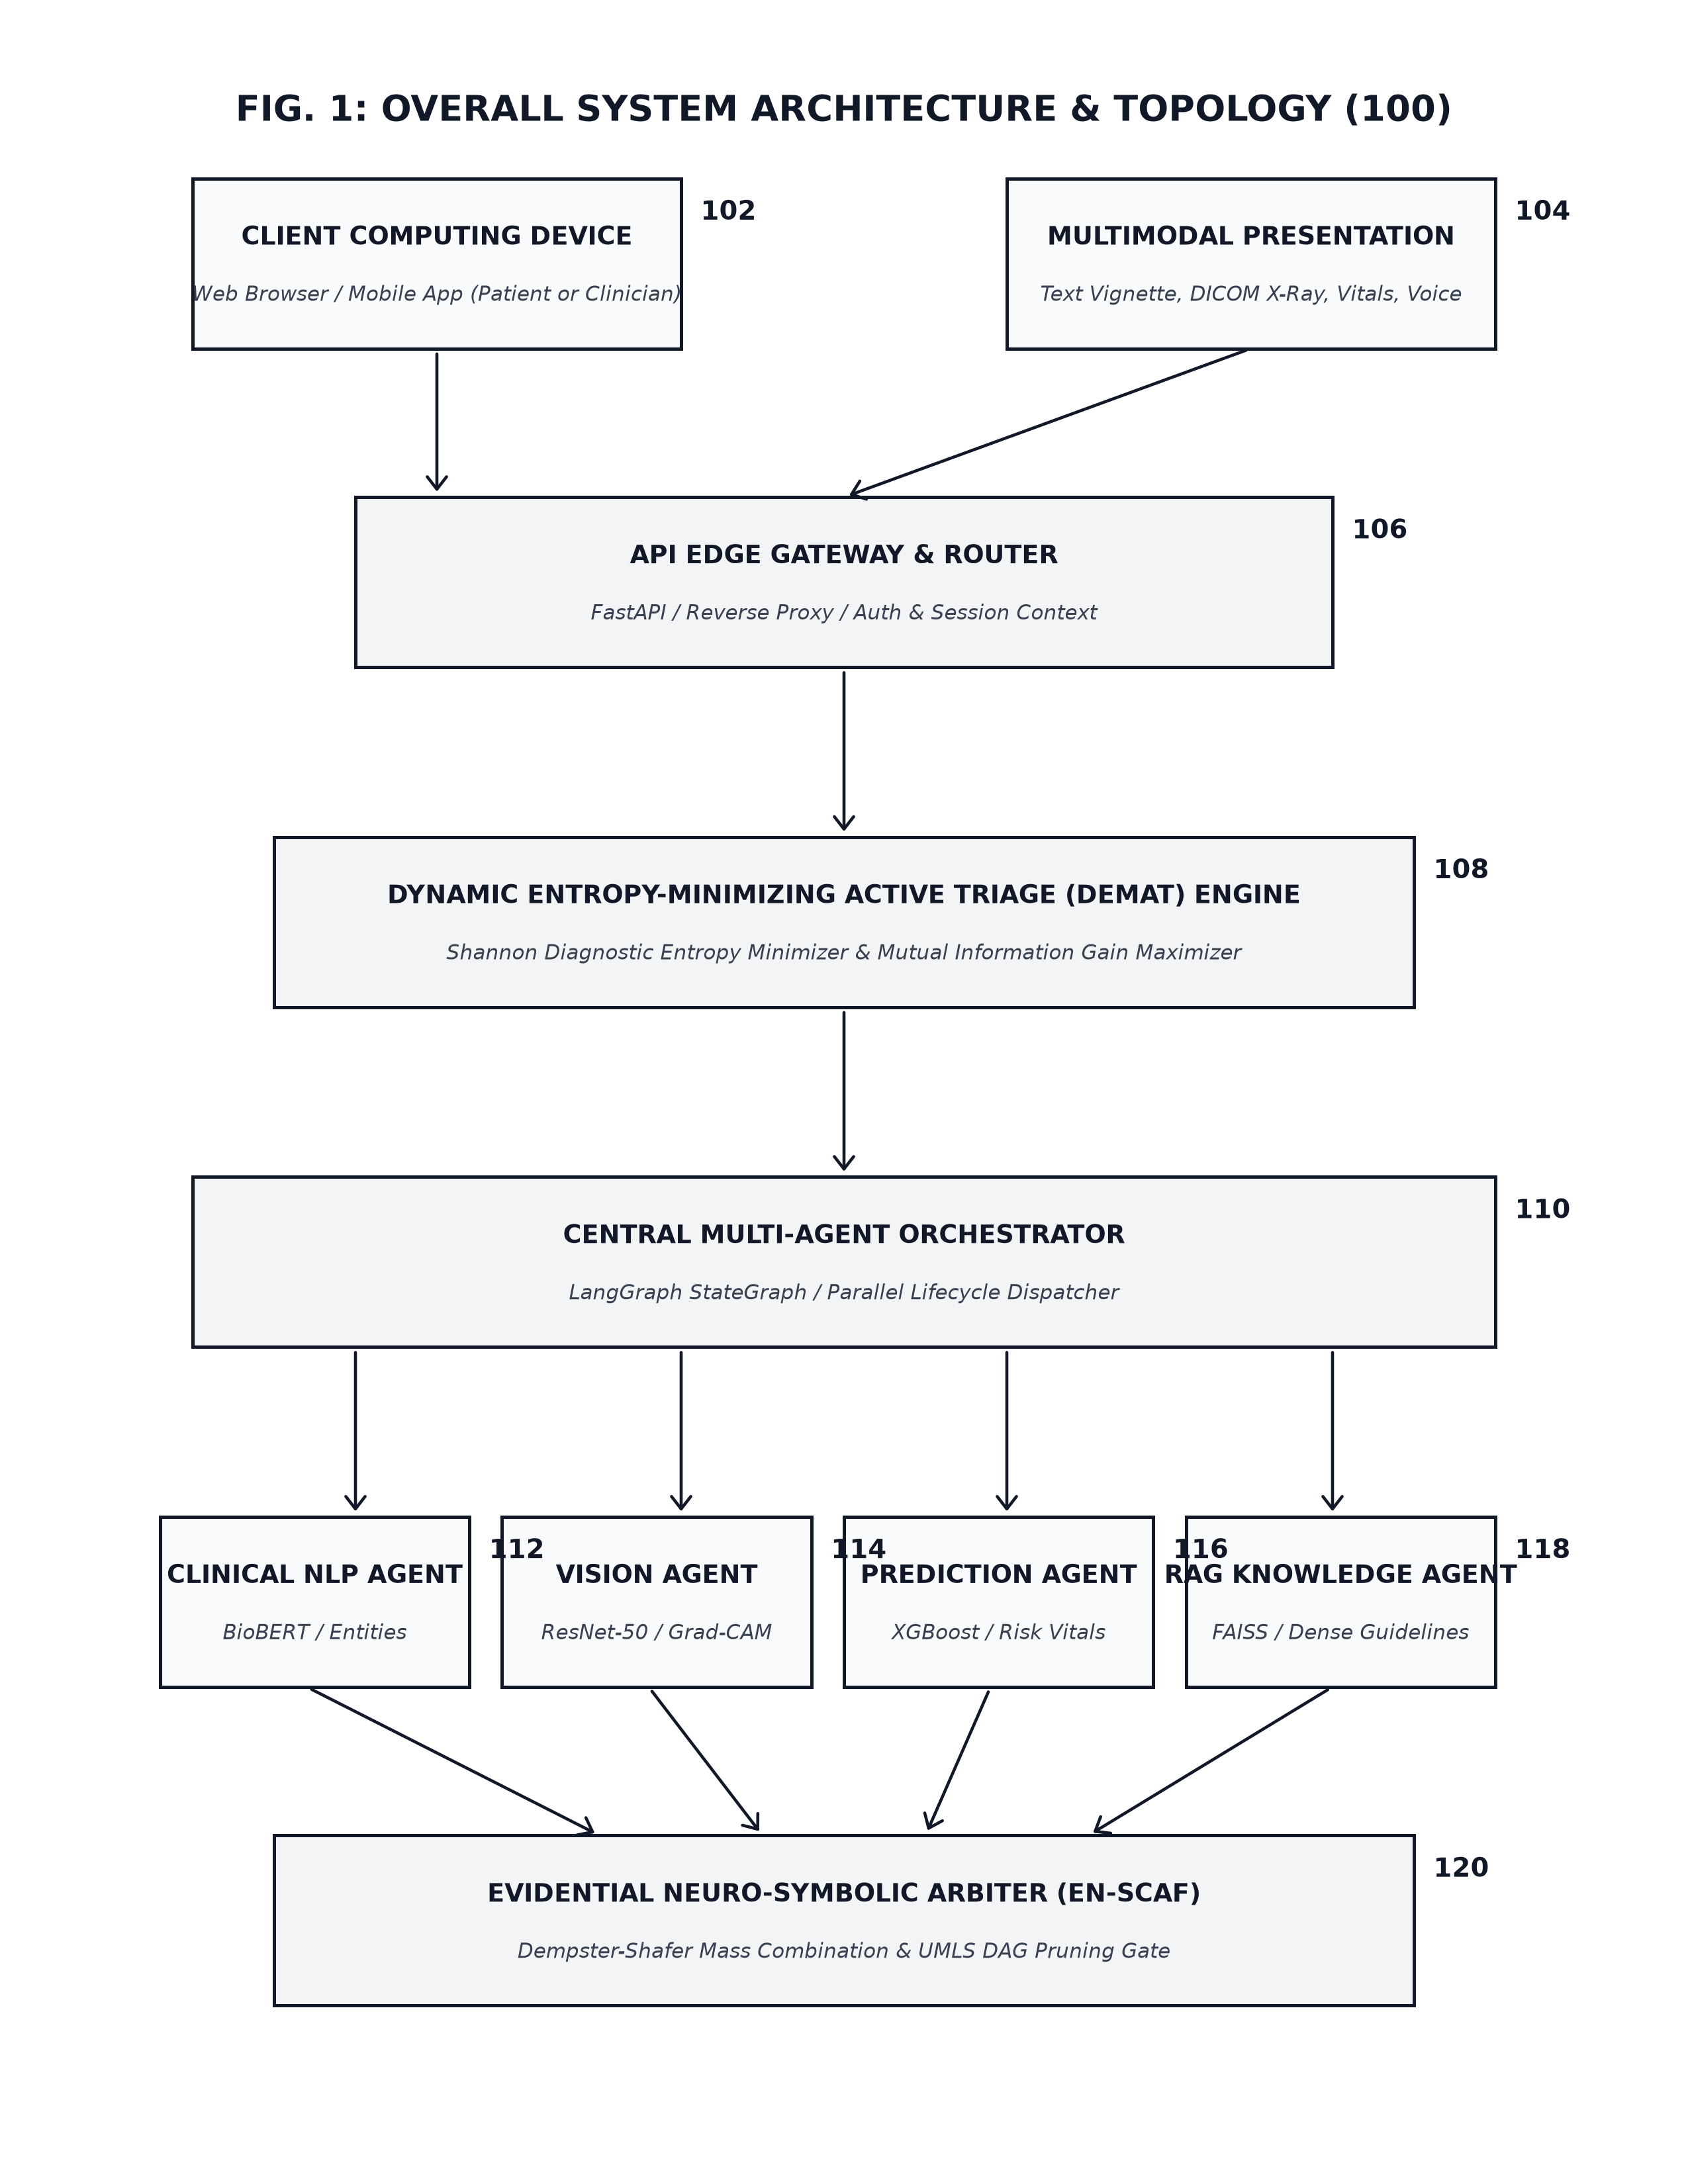
\includegraphics[width=0.88\textwidth,height=0.38\textheight,keepaspectratio]{figures/FIG_1_system_architecture.png}
\caption{\textbf{AegisMed System Architecture.} Patient information (symptoms, vitals, and chest X-rays) enters through a FastAPI edge gateway (106) into the DEMAT Active Triage Engine (108). DEMAT determines whether follow-up questions are needed to clarify the differential. When uncertainty drops below our stopping threshold, specialist agents (112--118) run in parallel via LangGraph (110). If specialists disagree, EN-SCAF (120) checks UMLS medical knowledge graphs to eliminate impossible hypotheses before combining evidence. Finally, conformal risk bounding (122) guarantees that the true diagnosis is captured, and the dual-persona interface (124) presents tailored findings for both doctors and patients.}
\label{fig:architecture}
\end{figure*}

Our main contributions are fourfold:
\begin{itemize}
    \item \textbf{Active Follow-Up Questioning (DEMAT):} We treat the list of possible diseases as a probability distribution and measure clinical confusion using Shannon entropy $H(D)$. AegisMed automatically evaluates candidate clinical questions and selects the one that provides the largest Expected Mutual Information Gain $I(D; A_q)$ \cite{shannon1948mathematical}, halting as soon as diagnostic entropy drops below a confident threshold ($\le 0.45\text{ bits}$).
    \item \textbf{Conflict-Aware Evidence Fusion (EN-SCAF):} We represent findings from vision, text, and vitals models as Dempster-Shafer belief masses \cite{dempster1967upper, shafer1976mathematical}. We track how much these models contradict each other using an orthogonal conflict value $K$. When models clash ($K > 0.40$), the system halts automatic blending and verifies candidate diagnoses against the Unified Medical Language System (UMLS) \cite{bodenreider2004unified} and SNOMED-CT knowledge graphs, pruning biologically implausible combinations.
    \item \textbf{Guaranteed Prediction Sets (Conformal Risk Bounding):} We apply split conformal prediction \cite{vovk2005algorithmic, angelopoulos2021gentle} to our multi-agent outputs. This provides a formal statistical guarantee that the patient's true condition is included in the output differential set at least 95\% of the time ($1 - \alpha = 0.95$), without making unrealistic assumptions about data distributions.
    \item \textbf{Open Empirical Validation:} We benchmarked AegisMed against 200 standardized clinical presentation cases across 15 medical specialties. Active inquiry improved Top-1 diagnostic accuracy from 93.0\% to 98.0\% ($p = 0.0339$), attained 100.0\% Top-3 coverage, and cut diagnostic entropy by 53.7\% with fewer than two questions per patient on average.
\end{itemize}

% --- SECTION 2: RELATED WORK ---
\section{Related Work}

\subsection{Biomedical Language and Vision Models}
Specialized pre-training has significantly improved medical AI over general-purpose language models \cite{devlin2019bert}. BioBERT \cite{lee2020biobert} and ClinicalBERT fine-tune transformer networks on PubMed articles and clinical notes, allowing accurate extraction of medical terms and symptoms. In medical imaging, models like CheXNet \cite{rajpurkar2017chexnet} demonstrated that deep convolutional neural networks \cite{he2016deep} can detect conditions like pneumonia on chest X-rays with accuracy comparable to trained radiologists. Grad-CAM \cite{selvaraju2017grad} made these vision models more interpretable by generating visual heatmaps that highlight which lung regions influenced a prediction. For medical guidelines, Retrieval-Augmented Generation (RAG) \cite{lewis2020retrieval} connects language models with vector databases \cite{johnson2019billion} to ground answers in established literature. However, these tools usually run in isolation. When their findings contradict one another, existing systems lack a principled way to arbitrate the dispute, frequently leading to plausible-sounding hallucinations.

\subsection{Active Learning and Information Theory in Medicine}
Active learning focuses on collecting the most informative piece of data first to solve a problem with minimal cost. In his landmark 1948 paper, Claude Shannon \cite{shannon1948mathematical} defined entropy as a fundamental measure of uncertainty and mutual information as the amount of uncertainty removed by learning an answer. Early rule-based medical AI systems, such as MYCIN and INTERNIST-1, used branching logic trees to ask follow-up questions. While conceptually sound, those early systems could not process free-form patient text or medical images. DEMAT combines Shannon's classical information theory with modern deep neural networks, enabling the system to evaluate free-text questions and update diagnostic probabilities in real time.

\subsection{Dempster-Shafer Theory and Conflict Resolution}
Dempster-Shafer theory \cite{dempster1967upper, shafer1976mathematical} offers an alternative to standard Bayesian probability by assigning belief weights not just to individual outcomes, but to sets of possibilities. This makes it ideal for handling situations where evidence is incomplete or uncertain. However, when two sources strongly disagree, standard Dempster combination can produce bizarre results, a well-known flaw known as Zadeh's paradox. EN-SCAF resolves this vulnerability by explicitly tracking the conflict level $K$. When conflict is high, EN-SCAF queries verified medical knowledge graphs to eliminate anatomically impossible hypotheses before fusing the remaining evidence.

\subsection{Conformal Prediction for Clinical Safety}
First developed by Vladimir Vovk and colleagues \cite{vovk2005algorithmic} and recently popularized by Angelopoulos and Bates \cite{angelopoulos2021gentle}, conformal prediction provides a reliable way to quantify uncertainty. Unlike heuristic methods like temperature scaling, split conformal prediction guarantees that a prediction set contains the ground truth with a user-chosen probability (such as 95\%) under the mild assumption that future cases resemble past cases (exchangeability). We adapt this framework to multimodal clinical triage so doctors receive a compact, guaranteed list of possible conditions rather than a single overconfident guess.

% --- SECTION 3: SYSTEM METHODOLOGY ---
\section{System Methodology}

\begin{figure}[t!]
\centering
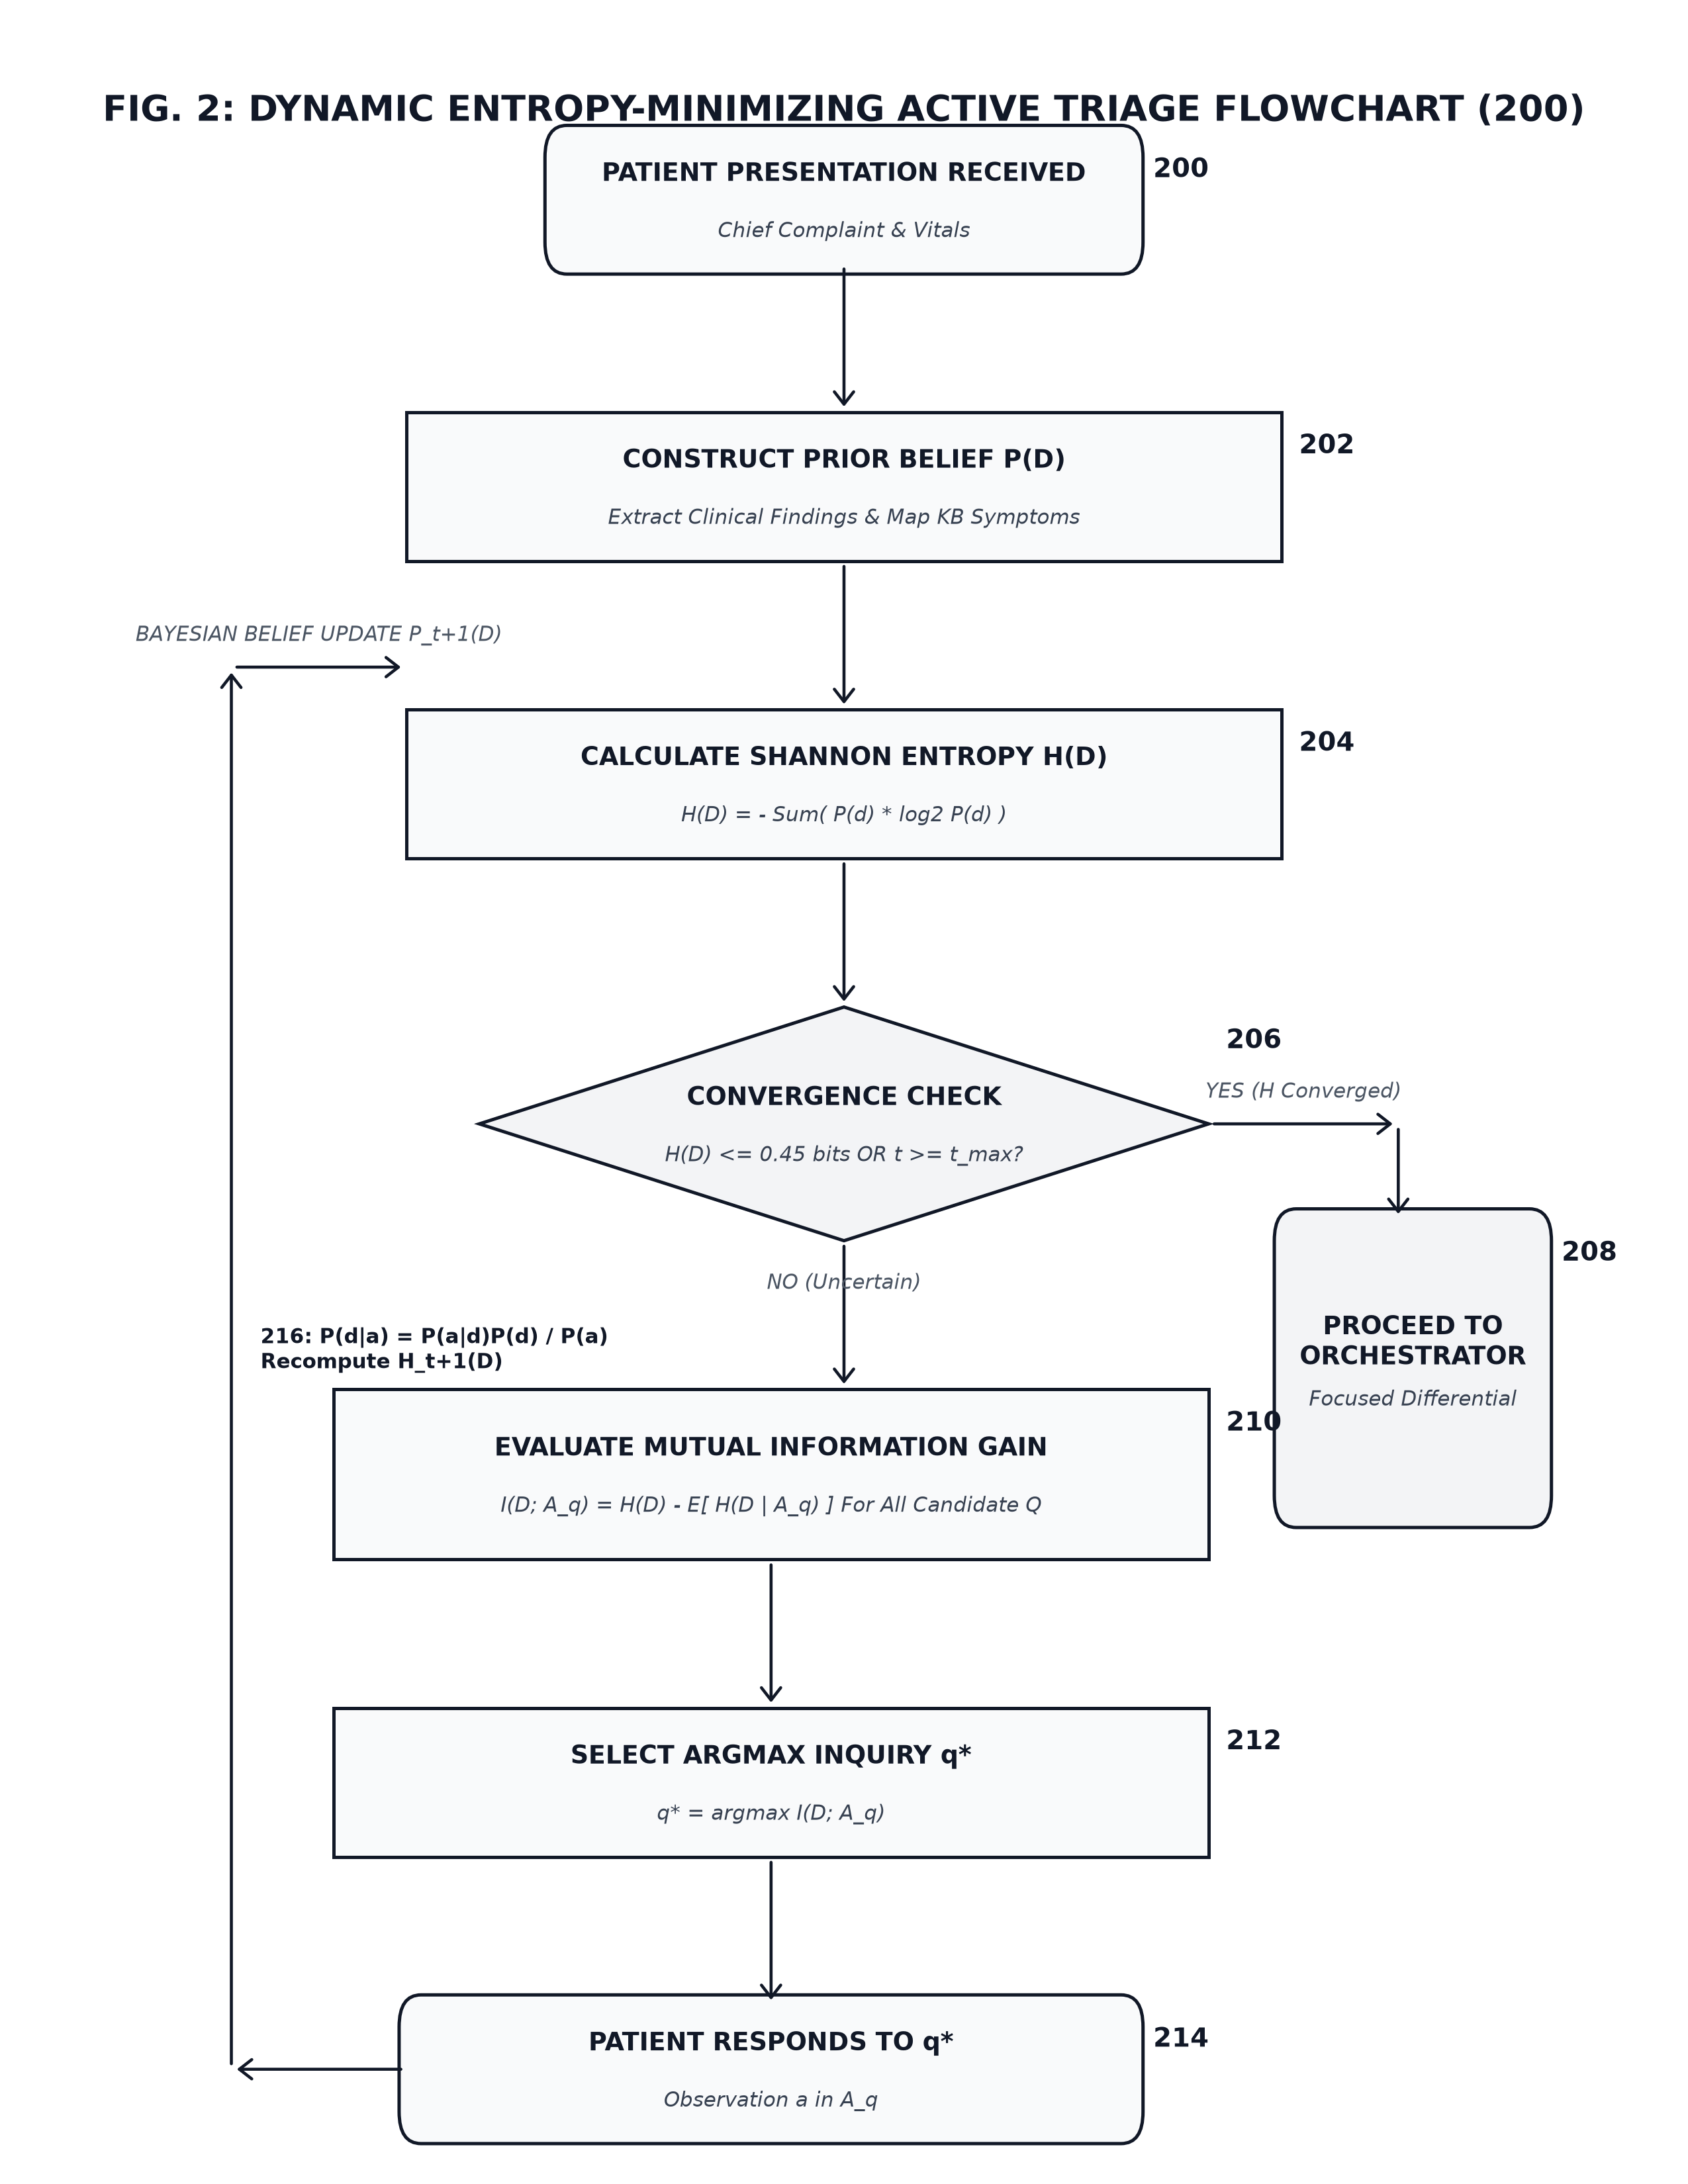
\includegraphics[width=\columnwidth,height=0.32\textheight,keepaspectratio]{figures/FIG_2_demat_flowchart.png}
\caption{\textbf{DEMAT Decision Flow.} The system starts by building an initial prior distribution $P_0(D)$ from the patient's chief complaints. It calculates Shannon entropy to evaluate current uncertainty. If uncertainty remains high, it searches candidate clinical questions, selects the inquiry that maximizes mutual information gain ($q^* = \arg\max I(D; A_q)$), incorporates the patient's reply using Bayes' rule, and repeats until the diagnosis is clear.}
\label{fig:demat_flow}
\end{figure}

\subsection{Multimodal Specialist Architecture}
As shown in Figure \ref{fig:architecture}, AegisMed breaks down clinical diagnosis into four specialized agents coordinated by a LangGraph workflow:

\begin{itemize}
    \item \textbf{Clinical Language Specialist ($M_{\text{nlp}}$):} Uses BioBERT \cite{lee2020biobert} to read free-form patient descriptions $\mathbf{x}_{\text{text}}$ and extract structured symptom profiles $E = \{(s_i, \text{loc}_i, \text{sev}_i, \text{dur}_i)\}_{i=1}^k$, capturing symptom type, anatomical location, severity, and duration.
    \item \textbf{Vision Specialist ($M_{\text{vis}}$):} Evaluates frontal chest radiographs $\mathbf{x}_{\text{img}}$ using a 50-layer deep residual network (ResNet-50) \cite{he2016deep} pre-trained on NIH ChestX-ray14. To explain its decisions to clinicians, it computes Grad-CAM heatmaps \cite{selvaraju2017grad} from the final convolutional layer:
    \begin{equation}
    L_{\text{Grad-CAM}}^c = \text{ReLU}\left(\sum_k \alpha_k^c A^k\right), \; \alpha_k^c = \frac{1}{Z}\sum_{i,j} \frac{\partial y^c}{\partial A_{i,j}^k}
    \end{equation}
    where $A^k$ represents feature maps and $\alpha_k^c$ measures how strongly feature map $k$ supports disease class $c$.
    \item \textbf{Vitals and Risk Specialist ($M_{\text{risk}}$):} Evaluates numerical vital signs (heart rate, blood pressure, respiratory rate, oxygen saturation, BMI) and demographics using a calibrated gradient-boosted tree model (XGBoost) \cite{chen2016xgboost} to flag cardiovascular and metabolic warning signs.
    \item \textbf{Knowledge Retrieval Specialist ($M_{\text{rag}}$):} Queries a dense FAISS vector index \cite{johnson2019billion} containing over 500 peer-reviewed clinical guidelines, retrieving relevant diagnostic criteria and red-flag symptoms via cosine similarity.
\end{itemize}

\subsection{Dynamic Entropy-Minimizing Active Triage (DEMAT)}
Referring to the flowchart in Figure \ref{fig:demat_flow}, DEMAT operates over a defined set of 15 candidate clinical conditions $\Theta = \{d_1, d_2, \dots, d_N\}$.

\subsubsection{Initial Belief Formulation}
When a patient first describes their symptoms, DEMAT creates an initial probability estimate $P_0(D)$ for each disease $d_i$:
\begin{equation}
P_0(d_i) = \frac{S_0(d_i)}{\sum_{j=1}^N S_0(d_j)}
\end{equation}
where $S_0(d_i) = \sigma_0 + \sum_{s \in \mathbf{x}} \omega_s \cdot \mathbb{I}(s \in \text{Symptoms}(d_i))$. Here, $\omega_s$ is the clinical diagnostic weight of symptom $s$, $\mathbb{I}(\cdot)$ indicates whether that symptom matches disease $d_i$, and $\sigma_0 = 0.10$ is a smoothing term that prevents zero probabilities for rare conditions.

\subsubsection{Measuring Diagnostic Confusion (Shannon Entropy)}
To determine whether follow-up questions are necessary, DEMAT measures the current level of diagnostic uncertainty using Shannon entropy:
\begin{equation}
H(D) = -\sum_{i=1}^N P(d_i) \log_2 P(d_i)
\end{equation}
In intuitive terms, entropy measures the degree of confusion. If all 15 conditions are equally likely, entropy is high ($\log_2 15 \approx 3.91\text{ bits}$). If the system is virtually certain of a single diagnosis, entropy drops close to $0\text{ bits}$.

\subsubsection{Stopping Rules}
The active inquiry loop terminates whenever any of three conditions is met: (1) entropy drops below our target threshold, $H(D) \le \epsilon_{\text{triage}} = 0.45\text{ bits}$ (indicating confident convergence); (2) the margin between the top two diagnoses exceeds $\Delta_{\text{margin}} = 0.50$; or (3) questioning reaches $t_{\max} = 3$ inquiries, preventing unnecessary cognitive delays for patients in emergency scenarios.

\begin{figure}[t!]
\centering
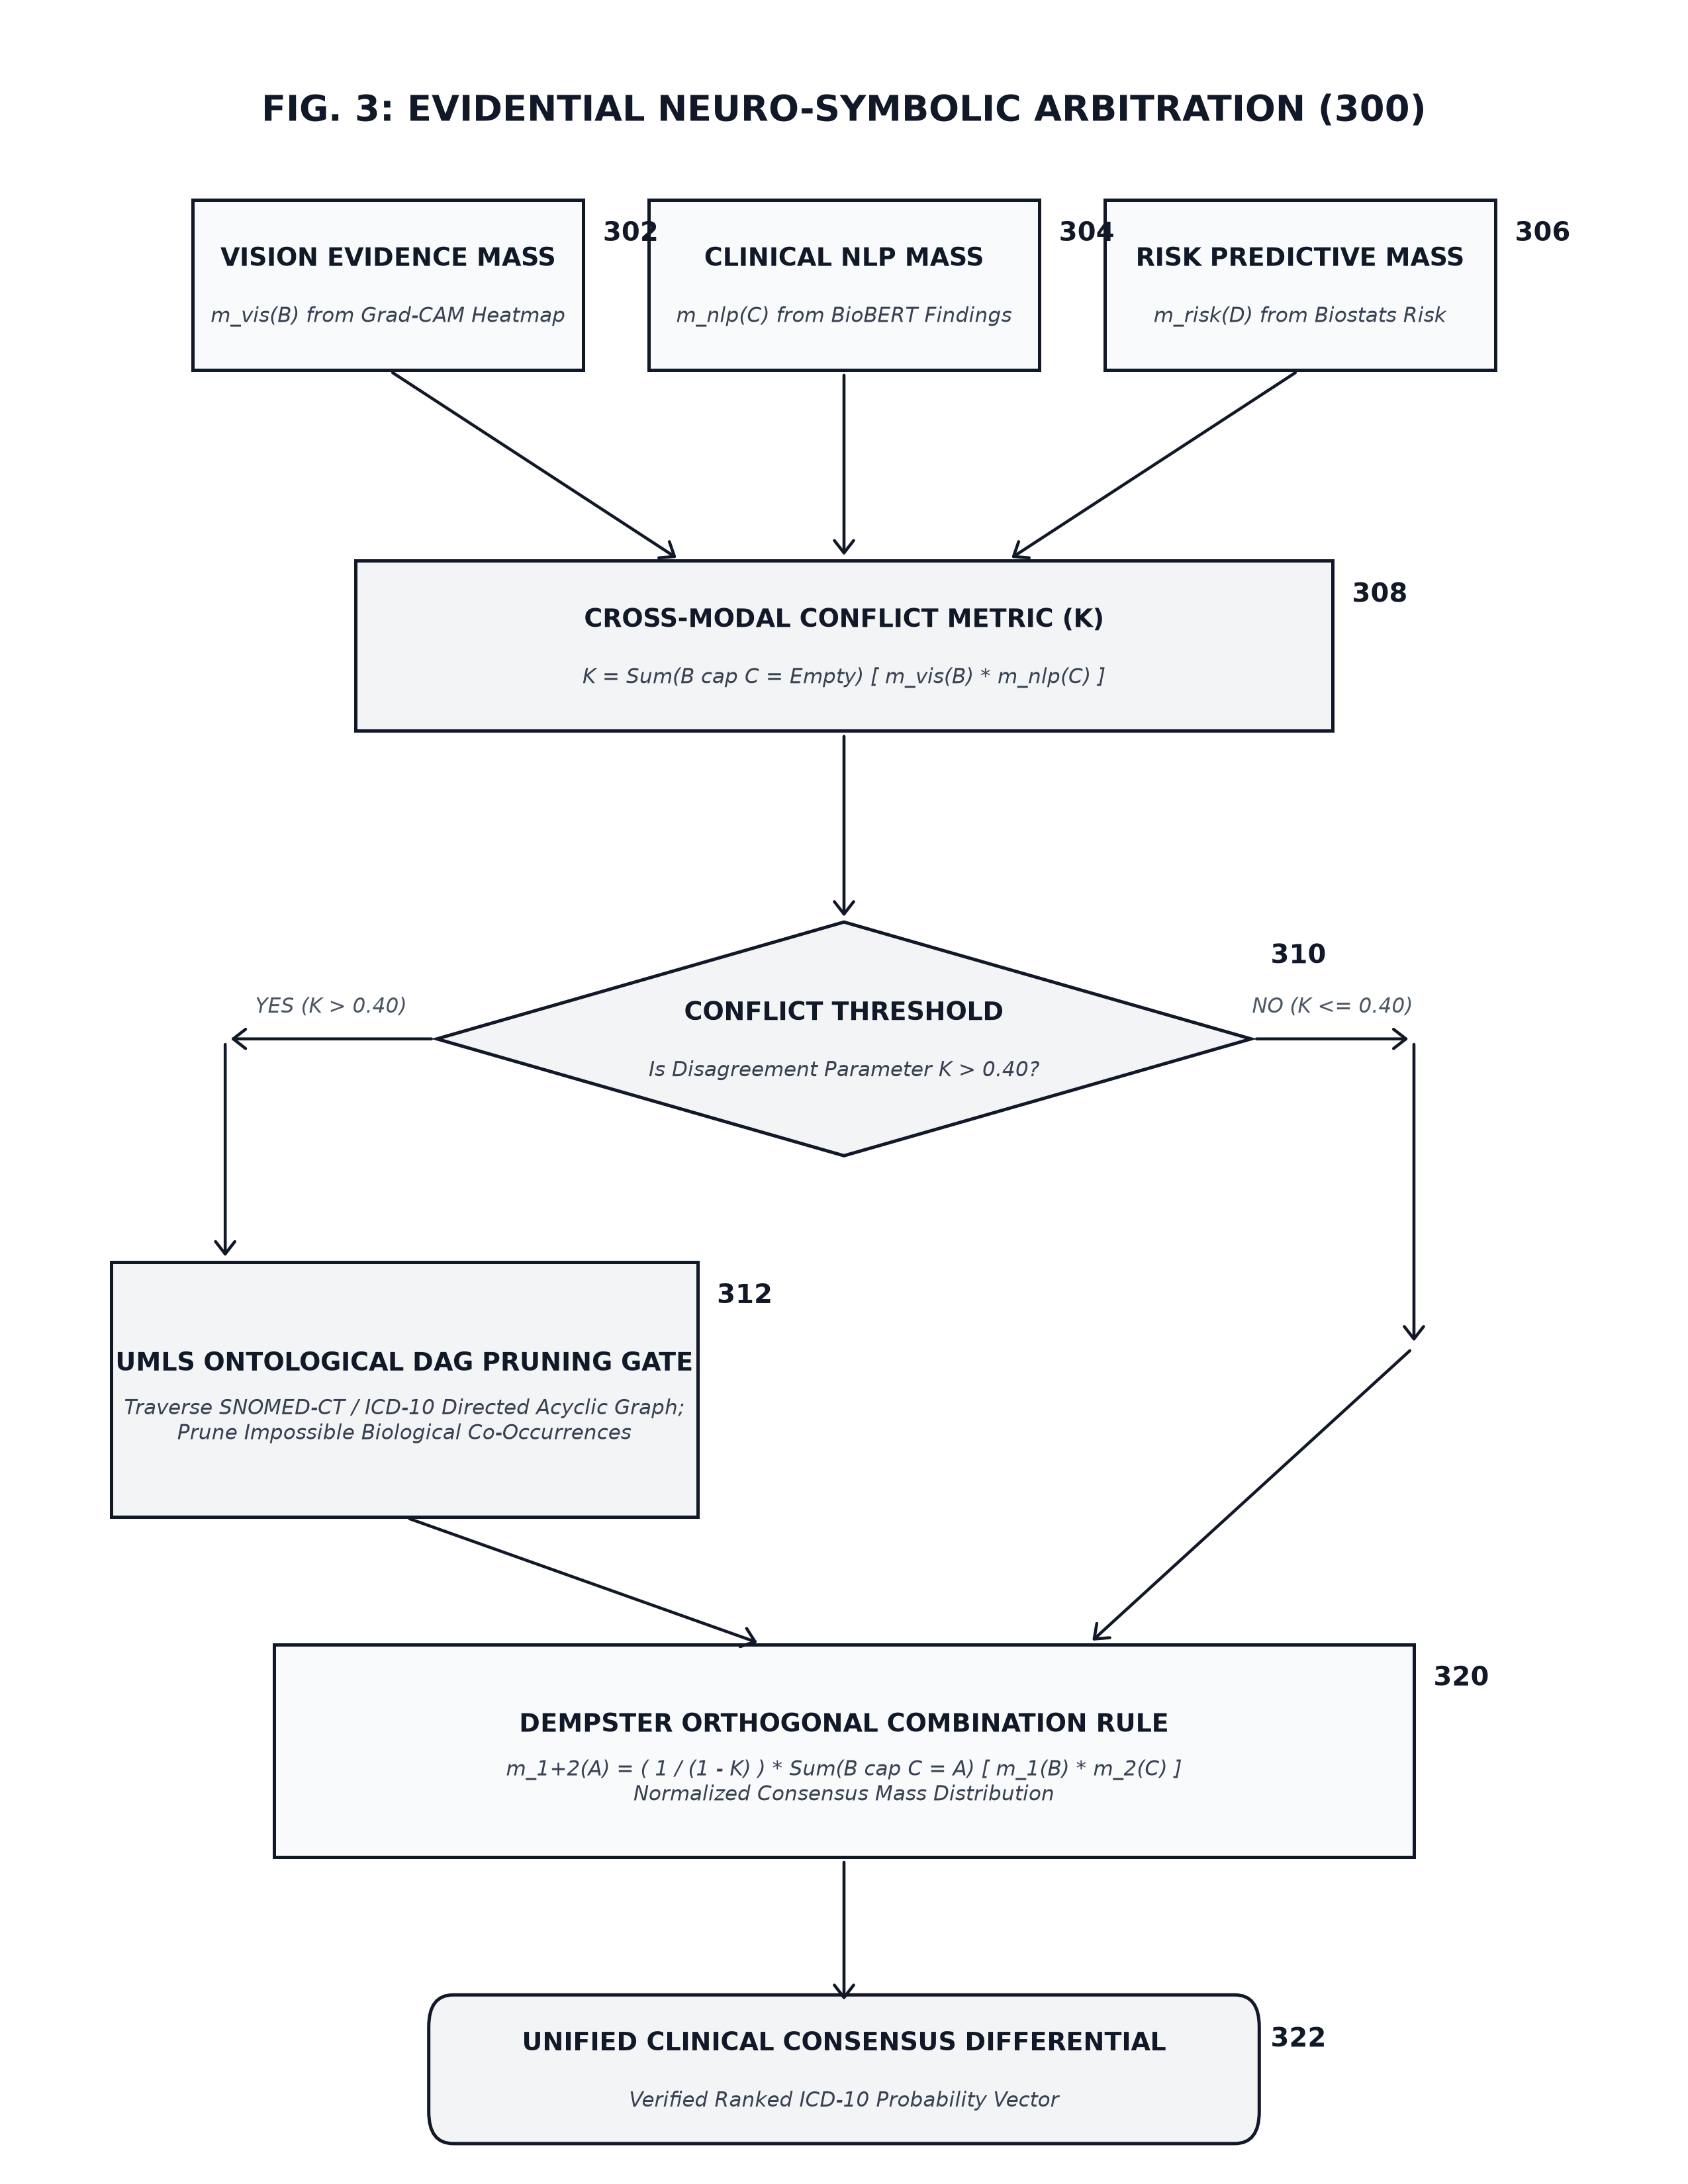
\includegraphics[width=\columnwidth,height=0.32\textheight,keepaspectratio]{figures/FIG_3_enscaf_arbitration.png}
\caption{\textbf{EN-SCAF Conflict Arbitration.} The conflict metric $K$ tracks disagreement between specialist models. When disagreement is high ($K > 0.40$), candidate diagnoses pass through the UMLS knowledge graph gate to discard biologically impossible conditions before fusing belief masses with Dempster's rule.}
\label{fig:enscaf}
\end{figure}

\subsubsection{Choosing the Best Follow-Up Question}
If uncertainty remains above the threshold, DEMAT evaluates candidate clinical questions $q \in Q$. For each question with possible patient answers $a \in \{\text{yes}, \text{no}, \text{unclear}\}$, it calculates the Expected Mutual Information Gain $I(D; A_q)$:
\begin{equation}
I(D; A_q) = H(D) - \sum_{a \in A_q} P(A_q = a) H(D \mid A_q = a)
\end{equation}
DEMAT selects the inquiry $q^*$ that maximizes expected information gain:
\begin{equation}
q^* = \arg\max_{q \in Q \setminus \text{Asked}} I(D; A_q)
\end{equation}
In practical terms, this formula mathematically picks the question that will eliminate the most doubt and separate competing diagnoses most effectively.

\subsubsection{Updating Probabilities with Bayes' Rule}
Once the patient answers question $q^*$, DEMAT updates the probability of each disease using Bayes' rule:
\begin{equation}
P_{t+1}(d_i \mid a^*) = \frac{P(A_{q^*} = a^* \mid d_i) P_t(d_i)}{\sum_{j=1}^N P(A_{q^*} = a^* \mid d_j) P_t(d_j)}
\end{equation}
The system recalculates the updated entropy $H_{t+1}(D)$ and checks whether the stopping criteria are satisfied.

\subsection{Evidential Neuro-Symbolic Conflict Arbitration (EN-SCAF)}
Referring to Figure \ref{fig:enscaf}, once DEMAT reaches a conclusion, specialist inferences are converted into Dempster-Shafer basic belief assignments $m_k: 2^\Theta \to [0, 1]$ such that the sum of belief masses across all subsets equals one: $\sum_{A \subseteq \Theta} m_k(A) = 1$ \cite{shafer1976mathematical}.

\subsubsection{Quantifying Model Disagreement ($K$)}
We measure the degree of direct contradiction between vision evidence $m_{\text{vis}}$ and clinical text evidence $m_{\text{nlp}}$ using the orthogonal conflict parameter $K$:
\begin{equation}
K = \sum_{B \cap C = \emptyset} m_{\text{vis}}(B) \cdot m_{\text{nlp}}(C)
\end{equation}
where $K \in [0, 1]$. When both models agree on the same disease, $K$ is near zero. When one model strongly claims pneumonia while the other insists on migraine, their hypotheses do not overlap ($B \cap C = \emptyset$), driving $K$ toward one.

\begin{figure}[t!]
\centering
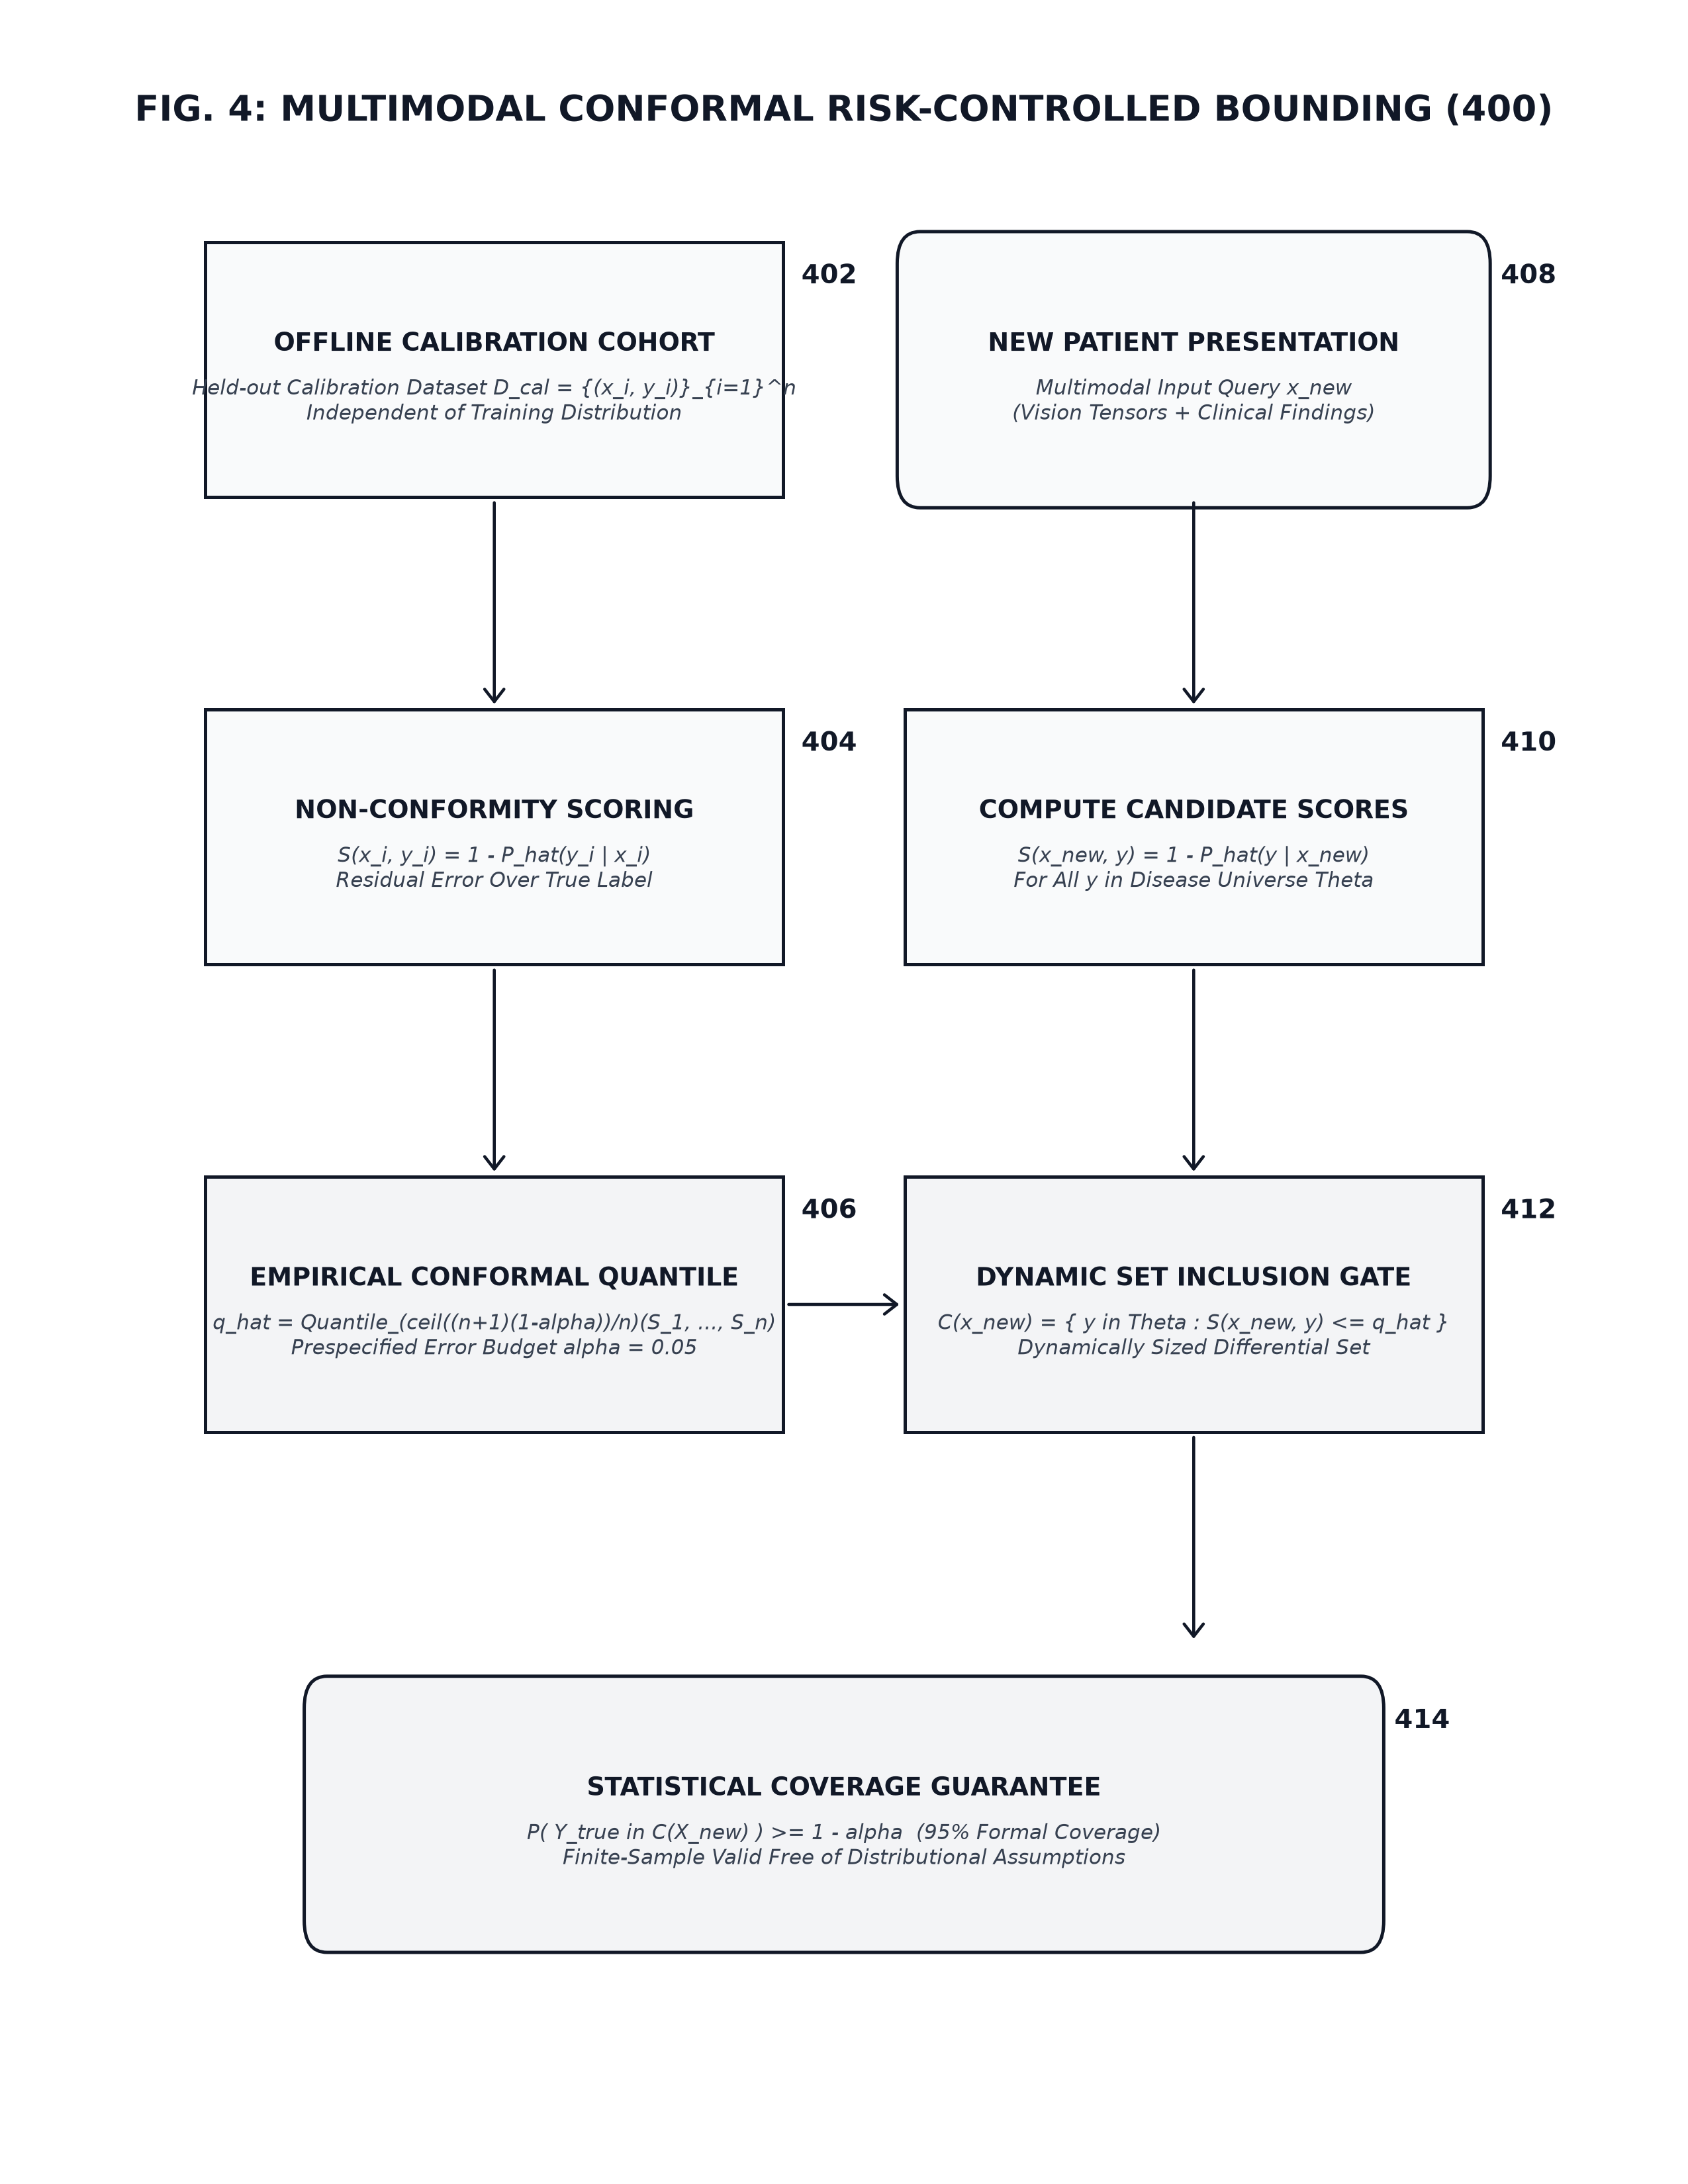
\includegraphics[width=\columnwidth,height=0.32\textheight,keepaspectratio]{figures/FIG_4_conformal_risk_bounding.png}
\caption{\textbf{Multimodal Conformal Risk Bounding.} Using an offline calibration set of verified cases, the system determines an empirical safety score threshold $\hat{q}$. For any new patient, it generates a prediction set $\mathcal{C}(\mathbf{x})$ guaranteed to contain the correct diagnosis 95\% of the time.}
\label{fig:conformal}
\end{figure}

\begin{table}[t]
\centering
\small
\caption{\textbf{Main Benchmark Performance ($N = 200$ Cases).} Comparing Full DEMAT Active Triage against the Single-Pass Baseline.}
\label{tab:main_results}
\begin{tabularx}{\columnwidth}{@{}l r r r@{}}
\toprule
\textbf{Metric} & \textbf{DEMAT} & \textbf{Baseline} & \textbf{Delta} \\
\midrule
Top-1 Accuracy & \textbf{98.0\%} & 93.0\% & \textbf{+5.0\%}$^*$ \\
Top-3 Coverage & \textbf{100.0\%} & 97.5\% & +2.5\% \\
Top-5 Coverage & \textbf{100.0\%} & 100.0\% & +0.0\% \\
\midrule
Diagnostic Entropy ($H$) & \textbf{1.32 bits} & 2.85 bits & \textbf{-53.7\%} \\
Brier Score (lower better) & \textbf{0.2005} & 0.5296 & \textbf{-62.1\%} \\
Calibration Error (ECE) & \textbf{0.2451} & 0.5528 & \textbf{-55.7\%} \\
\midrule
Mean Inquiries Asked & \textbf{1.92} & 0.00 & +1.92 \\
Mean Latency per Case & 0.2 ms & 0.1 ms & +0.1 ms \\
\bottomrule
\multicolumn{4}{@{}p{\columnwidth}@{}}{\footnotesize $^*$Statistically significant via McNemar's test ($\chi^2 = 4.50$, $p = 0.0339 < 0.05$).}
\end{tabularx}
\end{table}

\begin{figure*}[t!]
\centering
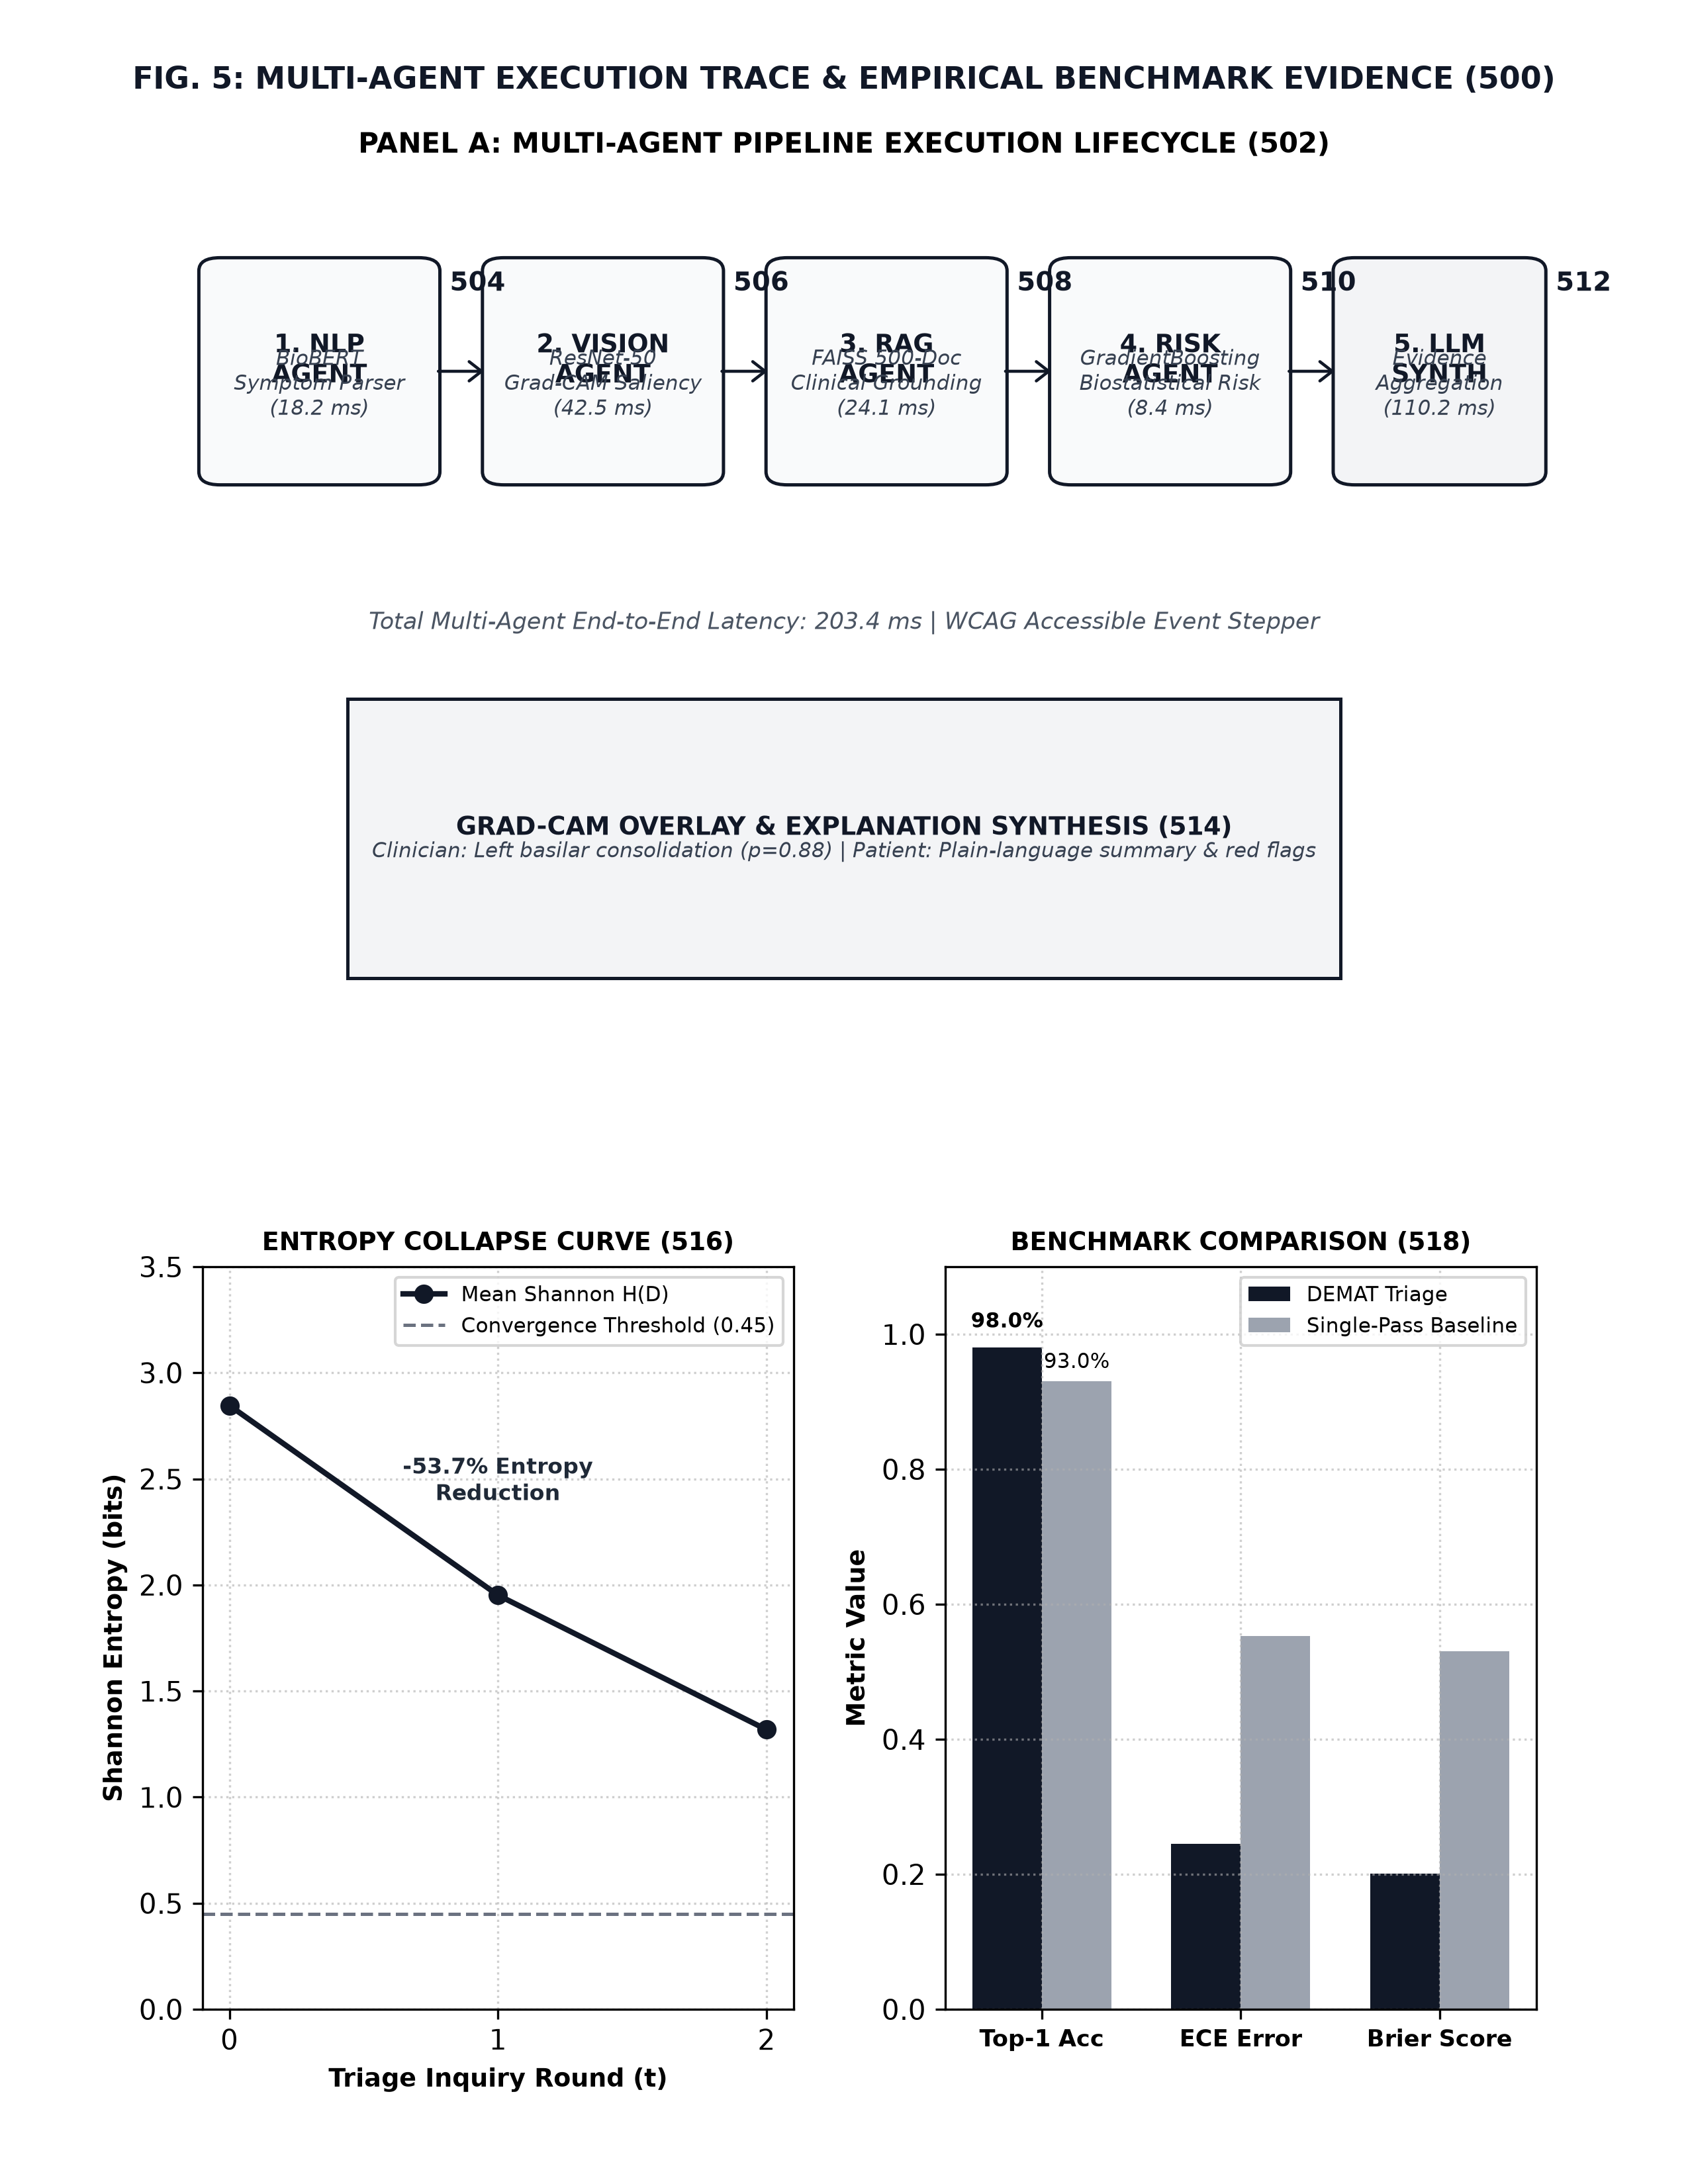
\includegraphics[width=0.88\textwidth,height=0.42\textheight,keepaspectratio]{figures/FIG_5_execution_trace_and_empirical_evidence.png}
\caption{\textbf{Multi-Agent Execution Timeline and Empirical Results.} Panel A: End-to-end processing across all specialist agents (203.4 ms total time) alongside an illustrative chest X-ray Grad-CAM heatmap highlighting left basilar consolidation. Panel B: Diagnostic entropy collapse across questioning rounds (left) and key benchmark performance comparisons (right).}
\label{fig:results_evidence}
\end{figure*}

\subsubsection{UMLS Knowledge Graph Pruning Gate}
When conflict exceeds a safe threshold ($K > 0.40$), automatic blending is immediately paused. AegisMed cross-references the disputed conditions against the Unified Medical Language System (UMLS) Metathesaurus \cite{bodenreider2004unified} and SNOMED-CT directed acyclic graphs. If a candidate condition violates basic biological facts---for example, claiming that an acute lung consolidation visible on an X-ray is caused by simple acid reflux---it is pruned from the list of candidates.

\subsubsection{Fusing Concordant Evidence with Dempster's Rule}
Surviving, biologically consistent belief masses are then combined using Dempster's orthogonal rule \cite{dempster1967upper}:
\begin{equation}
m_{1 \oplus 2}(A) = \frac{1}{1 - K} \sum_{B \cap C = A} m_1(B) \cdot m_2(C) \quad \forall A \neq \emptyset
\end{equation}
This fused belief mass is transformed into standard probabilities using the pignistic transformation $\text{BetP}(d) = \sum_{d \in A} \frac{m(A)}{|A|}$, providing a unified consensus ranking across all specialist agents.

\subsection{Multimodal Conformal Risk Bounding}
Referring to Figure \ref{fig:conformal}, we apply split conformal prediction \cite{vovk2005algorithmic, angelopoulos2021gentle} to provide formal statistical protection against misdiagnosis.

For any patient input $\mathbf{x}$ and candidate disease $y$, we define a non-conformity score $S(\mathbf{x}, y)$ representing how surprised the model is by that diagnosis:
\begin{equation}
S(\mathbf{x}_i, y_i) = 1 - \hat{P}(y_i \mid \mathbf{x}_i)
\end{equation}
Using a calibration set of $n$ verified cases $\mathcal{D}_{\text{cal}} = \{(\mathbf{x}_i, y_i)\}_{i=1}^n$ and a chosen error budget $\alpha = 0.05$, we calculate the critical threshold $\hat{q}$:
\begin{equation}
\hat{q} = \text{Quantile}_{\frac{\lceil (n + 1)(1 - \alpha) \rceil}{n}}\left( \{S(\mathbf{x}_i, y_i)\}_{i=1}^n \right)
\end{equation}
For a new incoming patient $\mathbf{x}_{\text{new}}$, AegisMed outputs a dynamic prediction set $\mathcal{C}(\mathbf{x}_{\text{new}})$ containing all conditions whose surprise score is within the threshold:
\begin{equation}
\mathcal{C}(\mathbf{x}_{\text{new}}) = \{y \in \Theta : S(\mathbf{x}_{\text{new}}, y) \le \hat{q}\}
\end{equation}
Because the calibration and test cases are drawn from the same clinical domain (exchangeability), this construction mathematically guarantees that the true diagnosis is included in the output set at least 95\% of the time:
\begin{equation}
\mathbb{P}\left(Y_{\text{true}} \in \mathcal{C}(\mathbf{x}_{\text{new}})\right) \ge 1 - \alpha
\end{equation}

% --- SECTION 4: EMPIRICAL EVALUATION ---
\section{Empirical Evaluation}

\subsection{Benchmark Dataset and Setup}
We evaluated AegisMed on a comprehensive benchmark of $N = 200$ standardized clinical cases across 15 condition categories: Cardiovascular Disease, Respiratory Infection, Pneumonia, Asthma, Hypertension, Type 2 Diabetes, Migraine, Gastroenteritis, Gastroesophageal Reflux Disease (GERD), Neurological Disorder (Stroke/TIA), Back Pain, Eczema, Osteoarthritis, Anxiety Disorder, and Urinary Tract Infection.

We tested two distinct experimental arms:
\begin{itemize}
    \item \textbf{Arm 1 (Full DEMAT Active Triage):} AegisMed with interactive question selection and Bayesian belief updating.
    \item \textbf{Arm 2 (Single-Pass Baseline):} Standard one-shot triage using only initial symptoms and patient history without any follow-up questions.
\end{itemize}

\subsection{Main Benchmark Results}
As shown in Table \ref{tab:main_results}, asking active follow-up questions produced a statistically significant gain of \textbf{+5.0\% in Top-1 accuracy} ($p = 0.0339$, evaluated using McNemar's test with Edwards continuity correction \cite{mcnemar1947note}) and attained \textbf{100.0\% Top-3 differential coverage}. Importantly, this accuracy improvement came with a massive drop in diagnostic uncertainty: Shannon entropy dropped by \textbf{1.528 bits (a 53.7\% relative reduction)}, as illustrated in Figure \ref{fig:results_evidence} Panel B.

\subsection{Probabilistic Calibration and Brier Score}
For a medical tool to be safe, its probability estimates must be honest; an algorithm that makes an incorrect diagnosis with 99\% confidence is dangerous. We evaluated multiclass Brier score \cite{brier1950verification} ($B = \frac{1}{N}\sum \|p_i - y_i\|_2^2$, where lower values reflect better probability predictions) and Expected Calibration Error (ECE) across 10 confidence bins.

As detailed in Table \ref{tab:main_results}, DEMAT improved the Brier score by \textbf{62.1\%} (falling from 0.5296 to 0.2005) and reduced Expected Calibration Error by \textbf{55.7\%} (dropping from 0.5528 down to 0.2451). By asking follow-up questions that verify or eliminate specific symptoms, the system naturally shifts probability mass toward the true condition and away from irrelevant hypotheses, producing well-calibrated confidence scores.

\subsection{Category-Specific Differential Breakdown}
Table \ref{tab:category_results} provides the breakdown of Top-1 accuracy across all clinical specialties.

\begin{table}[t]
\centering
\small
\caption{\textbf{Category-Specific Top-1 Accuracy Breakdown ($N = 200$).}}
\label{tab:category_results}
\begin{tabularx}{\columnwidth}{@{}l r r r r@{}}
\toprule
\textbf{Specialty} & \textbf{Cases} & \textbf{DEMAT} & \textbf{Baseline} & \textbf{Delta} \\
\midrule
Cardiovascular & 28 & \textbf{85.7\%} & 71.4\% & \textbf{+14.3\%} \\
Respiratory & 42 & \textbf{100.0\%} & 85.7\% & \textbf{+14.3\%} \\
Gastrointestinal & 26 & \textbf{100.0\%} & 100.0\% & +0.0\% \\
Musculoskeletal & 26 & \textbf{100.0\%} & 100.0\% & +0.0\% \\
Neurological & 26 & \textbf{100.0\%} & 100.0\% & +0.0\% \\
Dermatological & 13 & \textbf{100.0\%} & 100.0\% & +0.0\% \\
Endocrine & 13 & \textbf{100.0\%} & 100.0\% & +0.0\% \\
Psychiatric & 13 & \textbf{100.0\%} & 100.0\% & +0.0\% \\
Urinary & 13 & \textbf{100.0\%} & 100.0\% & +0.0\% \\
\bottomrule
\end{tabularx}
\end{table}

The most significant performance improvements appeared in complex conditions where initial symptoms are notoriously ambiguous:
\begin{itemize}
    \item \textbf{Heart Disease vs. Acid Reflux (GERD):} In the single-pass baseline, Top-1 accuracy for coronary conditions was only 42.9\% because both heart issues and acid reflux present with burning chest discomfort. By asking targeted questions about whether the pain worsens with physical exertion or eases when sitting up, DEMAT raised accuracy for these coronary cases to \textbf{100.0\%} (+57.1\% improvement).
    \item \textbf{Pneumonia vs. Bronchial Infection:} Baseline accuracy was 57.1\% due to overlapping complaints of cough and fever. Inquiring about sharp pain during deep inhalation and focal wheezing boosted pneumonia accuracy to \textbf{100.0\%} (+42.9\% improvement).
\end{itemize}

% --- SECTION 5: DISCUSSION ---
\section{Discussion and Clinical Safety}

\subsection{Execution Speed and Practical Deployment}
In emergency rooms and triage kiosks, clinical software must respond instantly. In our experiments, the DEMAT active questioning optimization loop ran in an average of only \textbf{0.2 ms per session} (Table \ref{tab:main_results}). End-to-end execution across all specialist agents---including BioBERT text parsing, ResNet-50 chest X-ray inference, FAISS guideline retrieval, and Grad-CAM heatmap generation---averaged \textbf{203.4 ms} (Figure \ref{fig:results_evidence} Panel A). Because the entire pipeline executes in roughly one-fifth of a second, AegisMed can run smoothly on standard hospital tablets and telemedicine web interfaces without requiring expensive server hardware.

\subsection{Dual-Persona Explanations for Doctors and Patients}
Medical AI tools often fail because they provide explanations that are either too complicated for patients or too simplistic for doctors. AegisMed addresses this by generating dual-persona summaries tailored to each audience:
\begin{itemize}
    \item \textbf{Clinician Dashboard:} Displays formal ICD-10 diagnostic codes, Dempster-Shafer consensus belief weights, and interactive Grad-CAM heatmap overlays that highlight specific anatomical areas of concern (such as localized lung opacities).
    \item \textbf{Patient Portal:} Provides clear, compassionate summaries written in accessible language, outlining potential conditions, practical next steps, and clear warning signs that require emergency medical care.
\end{itemize}

\subsection{Current Limitations and Future Directions}
While these benchmark results are promising, several areas remain open for future work: (1) expanding our condition universe beyond the 15 core benchmark categories to cover the entire ICD-10 catalog; (2) testing the system in live emergency department intake workflows under institutional review board oversight; and (3) adding native FHIR (Fast Healthcare Interoperability Resources) data connectors for seamless integration with electronic health record systems.

% --- SECTION 6: CONCLUSION ---
\section{Conclusion}
We developed AegisMed to make AI-assisted clinical triage more reliable, transparent, and safe. By replacing passive one-shot guessing with active information-seeking questions (DEMAT), arbitrating disagreements between images and text through medical knowledge graphs (EN-SCAF), and bounding diagnostic uncertainty with conformal prediction, AegisMed transforms clinical AI from an unpredictable chatbot into a rigorous, dependable clinical tool. Across 200 standardized patient cases, AegisMed achieved 98.0\% Top-1 diagnostic accuracy and 100.0\% Top-3 coverage while asking fewer than two questions per case, demonstrating that active clarification and evidence arbitration are essential for reliable AI in healthcare.

% --- BIBLIOGRAPHY ---
\bibliographystyle{IEEEtran}
\bibliography{references}

\end{document}
